\chapter{Marco teórico} 
\label{Capitulo2} 
\lhead{\emph{Marco teórico}}
En este capítulo se da un repaso teórico de los temas relevantes dentro del proyecto.
%Dentro de este capítulo se tratará de brindar al lector con las bases literarias para la comprensión del capítulo 3 y 4. Se considera que el lector tiene conocimientos básicos de ingeníeria por lo que no se profundizará de forma extensa en cada uno de los temas.

\section{2.1 Imágenes espectrales} 
Las imágenes espectrales son aquellas que reproducen la figura de un objeto en función de la longitud de onda dentro del espectro electromagnético(vea Figura \ref{fNasa}) que esté reflejando (o emitiendo) el objeto en cuestión. Las cámaras ordinarias RGB captan aquellas ondas dentro de los canales rojo, verde y azul del espectro visible (vea tabla \ref{tEV}).
\subsection{2.1.1 Espectro electromagnético}
El espectro electromagnético es la distribución energética del conjunto de las ondas electromagnéticas, combinación de campos eléctricos y magnéticos oscilantes, transportándose a través del espacio de un lugar a otro. Se le da el nombre de electromagnético ya que se refiere al conjunto de vibraciones magnéticas y eléctricas, tal como se puede observar en la Figura \ref{fPropagacion}.

\begin{figure}[h]
  \centering
  \framebox[12cm]{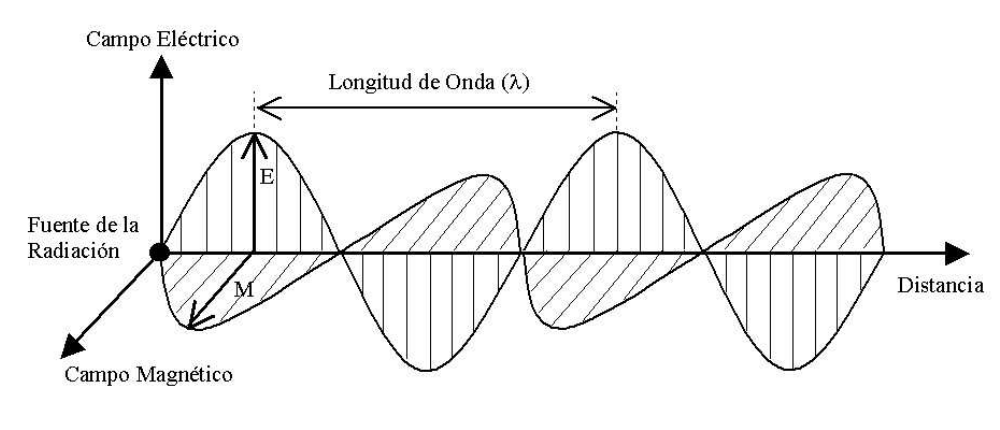
\includegraphics[width=.8\textwidth]{./images/propagacion.png}}
  \centering
  \caption{Se muestran los vectores eléctricos ($E$) y magnéticos ($M$), perpendiculares entre ellos,de una onda electromagnética. La longitud de onda ($\lambda$) corresponde a la distancia entre dos crestas consecutivas. \cite{chile}}
  \label{fPropagacion}
\end{figure}

Cuando se logra ver algo, no es directamente el objeto que se ve sino la radiación electromagnética dentro del rango visual que emite dicho objeto y parte de la energía es absorbida por el objeto, ya que actúan con base en los componentes químicos que lo forman. El espectro electromagnético se divide en rangos(vea tabla \ref{tEspectro}). 

También se le dice espectro electromagnético a la radiación electromagnética que absorbe o emite una sustancia. Dicha radiación sirve para identificar la sustancia de manera análoga a una huella dactilar lo cual será explicado en el siguiente subtema \ref{FirmasEspectrales}. Los espectros se pueden observar mediante espectroscopios que, además de permitir ver el espectro, permiten realizar medidas sobre el mismo, como son la longitud de onda, la frecuencia y la intensidad de la radiación.\\
Una cámara digital RGB tradicional capta el espectro visible que responde a longitudes de onda 390 nm a 750 nm(vea la tabla \ref{tEV}). El objetivo de las cámaras tradicionales es dar como resultado una imagen en el rango de visibilidad humana. Lo interesante es cuando tomamos en cuenta otros valores fuera del rango visible. (véase la Figura \ref{fNasa})

\begin{table}[]
\centering
\begin{tabular}{l|l|l|l|}
\cline{2-4}
                         & Color    & \begin{tabular}[c]{@{}l@{}}Intervalo de longitud\\ de onda ($\lambda$)\end{tabular} & \begin{tabular}[c]{@{}l@{}}Intervalo de \\ frecuencia ($\nu$)\end{tabular} \\ \cline{2-4} 
\cellcolor[HTML]{FE0000} & Rojo     & $\sim$ 700 - 635 nm                                                               & $\sim$ 430 - 480 THz                                                 \\ \cline{2-4} 
\cellcolor[HTML]{FFA500} & Naranja  & $\sim$ 635 – 590 nm                                                                & $\sim$ 480 – 510 THz                                                 \\ \cline{2-4} 
\cellcolor[HTML]{FFFF00} & Amarillo & $\sim$ 590 – 560 nm                                                                & $\sim$ 510 – 540 THz                                                 \\ \cline{2-4} 
\cellcolor[HTML]{008000} & Verde    & $\sim$ 560 – 520 nm                                                                & $\sim$ 540 – 580 THz                                                 \\ \cline{2-4} 
\cellcolor[HTML]{00FFFF} & Cian     & $\sim$ 520 – 490 nm                                                                & $\sim$ 580 – 610 THz                                                 \\ \cline{2-4} 
\cellcolor[HTML]{0000FF} & Azul     & $\sim$ 490 – 450 nm                                                                & $\sim$ 610 – 670 THz                                                 \\ \cline{2-4} 
\cellcolor[HTML]{EE82EE} & Violeta  & $\sim$ 450 – 400 nm                                                                & $\sim$ 670 – 750 THz                                                 \\ \cline{2-4} 
\end{tabular}
\caption{Espectro visible\cite{Craig}.}
\label{tEV}
\end{table}

\begin{table}[]
\centering
\begin{tabular}{|l|l|l|}
\hline
\multicolumn{1}{|c|}{\textbf{\begin{tabular}[c]{@{}c@{}}Región o Banda\\ Espectral\end{tabular}}} & \multicolumn{1}{c|}{\textbf{\begin{tabular}[c]{@{}c@{}}Longitud \\ de onda $\lambda$\end{tabular}}}         & \textbf{Características}                                                                                                                                                                                           \\ \hline
Rayos Gamma                                                                                       & \textless 0.03 nm                                                                                        & \multirow{2}{*}{\textit{\begin{tabular}[c]{@{}l@{}}Radiación completamente absorbida\\ por las capas superiores de la \\ atmósfera. No se utilizan en \\ teledetección.\end{tabular}}}                                                                                  \\ \cline{1-2}
\\Rayos X  \\                                                                                         & 0.03 - 30 nm                                                                                             &                                                                                                                                                                                                                                                                          \\ \hline
Ultravioleta (UV)                                                                                 & 0.03 - 0.4 $\mu$m                                                                                            & \textit{\begin{tabular}[c]{@{}l@{}}La radiación con $\lambda$ \textless 0.3 $\mu$m es\\ completamente absorbida por la capa\\ de ozono de la atmósfera.\end{tabular}}                                                                                                           \\ \hline
\begin{tabular}[c]{@{}l@{}}Visible (azul,verde\\ y rojo)\end{tabular}                             & \begin{tabular}[c]{@{}l@{}}0.4 - 0.5 $\mu$m (azul)\\ 0.5 - 0.6 $\mu$m (verde)\\ 0.6 - 0.7 $\mu$m (rojo)\end{tabular} & \textit{\begin{tabular}[c]{@{}l@{}}Se puede detectar a través de \\ fotodetectores y películas fotosensibles\\ normales (color B/N).\end{tabular}}                                                                                                                       \\ \hline
Infrarrojo reflejado                                                                              & \begin{tabular}[c]{@{}l@{}}0.7 - 1.3 $\mu$m \\ (IR cercano)\\ 1.3 - 3.0 $\mu$m \\ (IR medio)\end{tabular}        & \textit{\begin{tabular}[c]{@{}l@{}}Radiación solar reflejada que no\\ contiene información acerca de las\\ propiedades térmicas de los materiales.\\ El rango 0.7 a 0.9 $\mu$m se puede \\ detectar usando películas fotosensibles\\ (infrarrojo fotográfico).\end{tabular}} \\ \hline
Infrarrojo térmico                                                                                & \begin{tabular}[c]{@{}l@{}}3.0 - 5.0 um\\ 8.0 - 14.0 um\end{tabular}                                     & \textit{\begin{tabular}[c]{@{}l@{}}Corresponden a dos ventanas\\ atmosféricas en la región térmica.\end{tabular}}                                                                                                                                                        \\ \hline
\begin{tabular}[c]{@{}l@{}}Radar (región de \\ las microondas)\end{tabular}                       & 0.1 - 100 cm                                                                                             & \textit{\begin{tabular}[c]{@{}l@{}}Radiación de grandes longitudes de\\ onda, capaces de penetrar nubes,\\ nieblas y lluvia.\end{tabular}}                                                                                                                               \\ \hline
Ondas de Radio y TV                                                                               & \textgreater 100 cm                                                                                      & \textit{\begin{tabular}[c]{@{}l@{}}Radiación con las mayores longitudes\\ de onda del espectro. Se utilizan en \\ telecomunicaciones.\end{tabular}}                                                                                                                      \\ \hline
\end{tabular}
\caption{Descripción de las regiones del espectro electromagnético ($1 \mu m = 10^{-6}$ m y 1 nm = $10^{-9} m$)\cite{chile}.}
\label{tEspectro}
\end{table}
  

%Craig F. Bohren (2006). Fundamentals of Atmospheric Radiation: An Introduction with 400 Problems. Wiley-VCH. ISBN 3-527-40503-8.

\begin{figure}[h]
  \centering
  \framebox[14cm]{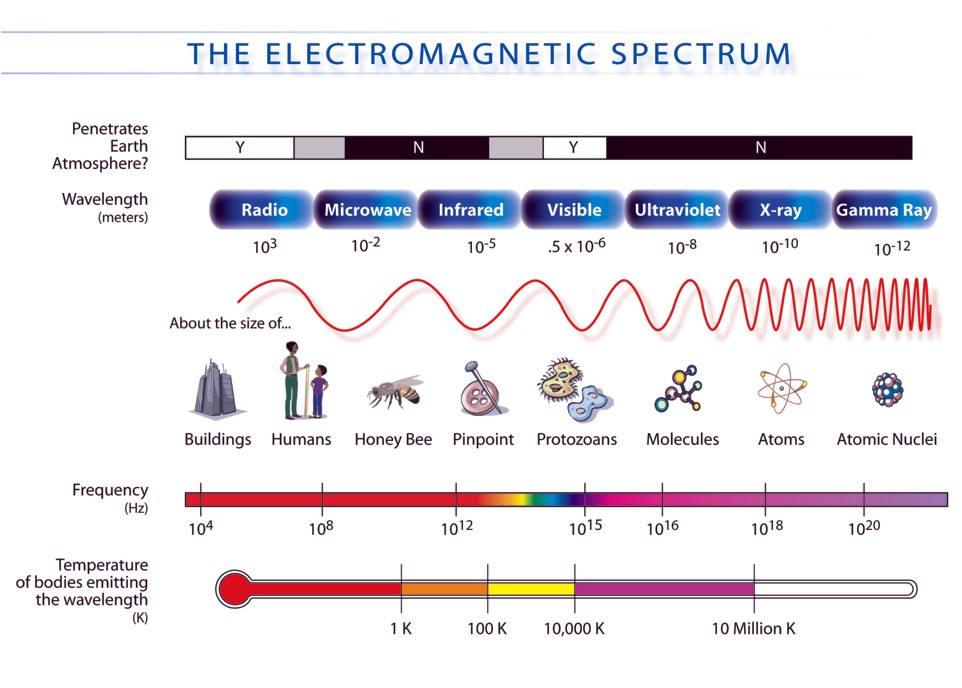
\includegraphics[width=.8\textwidth]{./images/nasa.jpg}}
  \centering
  \caption{Diagrama del espectro electromagnético \cite{nasaimage}.}
  \label{fNasa}
\end{figure}
\label{FirmasEspectrales}
\subsection{2.1.2 Firmas espectrales}
La firma espectral es la variación de reflectancia de la radiación proveniente de la energía solar cuando tiene contacto con la superficie terrestre reflejada, absorbida y transmitida. La energía es reflejada cuando es rebotada, es absorbida cuando conserva energía provocando calor en el material y es transmitida cuando pasa a través del material. Como se comentó en el capítulo anterior el espectro electromagnético es dado por la radiación emitida y absorvida por el objeto. Gracias a que cada elemento capturado emite radiación electromagnética recibida del sol de forma diferenciada, es posible mediante un análisis de los datos determinar que elementos químicos lo forman y determinar que es lo que se capto, tal como se puede ver en la Figura \ref{fFirma}.

\begin{figure}[h]
  \centering
  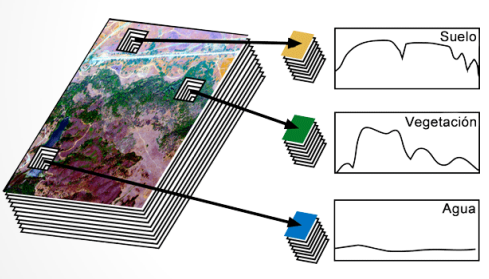
\includegraphics[width=.7\textwidth]{./images/firma.png}
  \centering
  \caption{Firmas espectrales de suelo, vegetación y agua. \cite{Quinones}.}
  \label{fFirma}
\end{figure}
%IMÁGENES HIPERESPECTRALES: ANÁLISIS Y APLICACIONES. Sebastián Quiñones F. Cartógrafo Centro de Ecología Aplicada
Otra de las aplicaciones muy comunes es detectar la sanidad de las plantas tomando en cuenta las variables ya mencionadas como se puede observar en un ejemplo en la Figura \ref{fSanidad}. También se han utilizado estas técnicas en detección de sanidad en animales \cite{animal} como se ve en la Figura \ref{fAnimal}.

\begin{figure}[h]
  \centering
  \framebox[14cm]{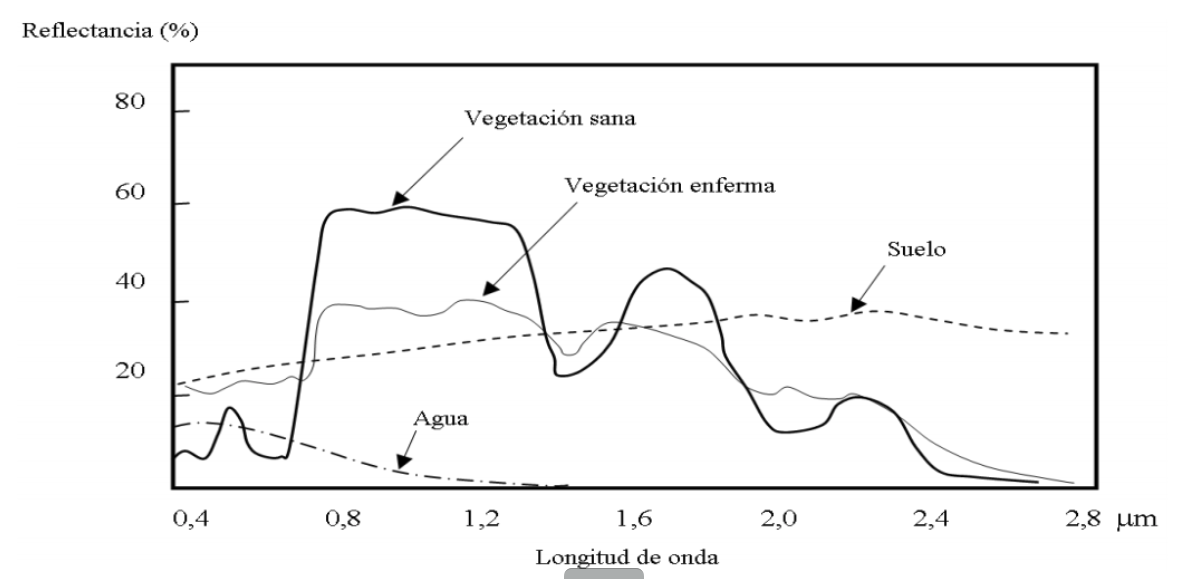
\includegraphics[width=.8\textwidth]{./images/sanidad.png}}
  \centering
  \caption{Detección de sanidad en vegetales \cite{chile}.}
  \label{fSanidad}
\end{figure}

\begin{figure}[h]
  \centering
  \framebox[5cm]{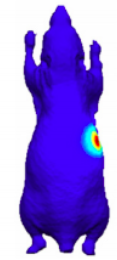
\includegraphics[width=.2\textwidth]{./images/animal.png}}
  \centering
  \caption{Detección espectral de anormalidades en animales. \cite{animal}.}
  \label{fAnimal}
\end{figure}
%Abhijit J Chaudhari and Felix Darvas and James R Bading and Rex A Moats and Peter S Conti and Desmond J Smith and Simon R Cherry and Richard M Leahy, “Hyperspectral and multispectral bioluminescence optical tomography for small animal imaging,” in Physics in Medicine and Biology, vol. 50, 2005 
\subsection{2.1.3 Imagen espectral}
Tomando en cuenta que una imagen es la reproducción de una figura por la combinación de los rayos de luz y que el espectro es la radiación electromagnética que es absorbida o emitida, podemos concluir que una imagen espectral es la reproducción de una figura de un objeto por la combinación de radiación emitida en cierta longitud de onda electromagnética (véase la Figura \ref{fWiki}).

\begin{figure}[h]
  \centering
  \framebox[14cm]{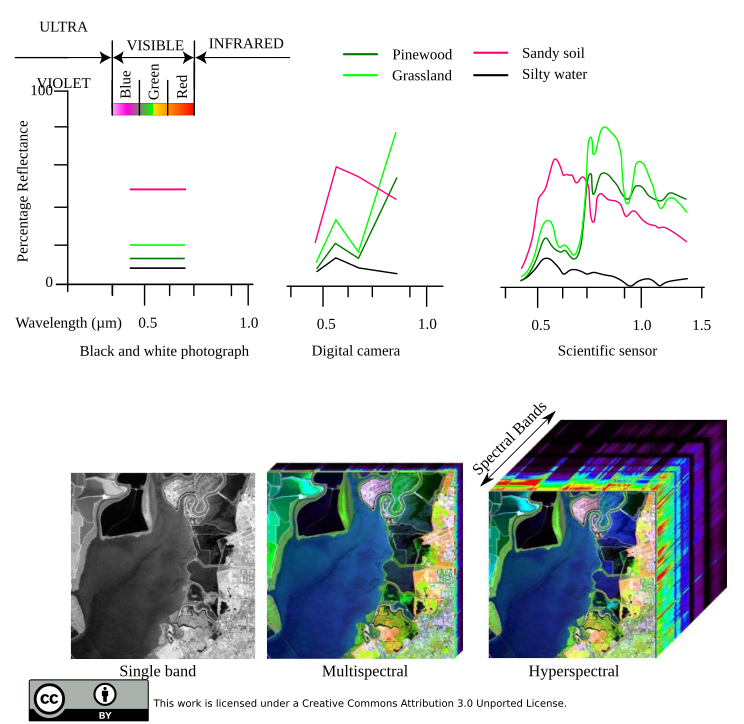
\includegraphics[width=.8\textwidth]{./images/wiki.png}}
  \centering
  \caption{Imagen hiperespectral, multiespectral y espectral.}
  \label{fWiki}
\end{figure}

\subsection{2.1.4 Imagen Multiespectral}
Las imágenes Multiespectrales son un conjunto de entre 3 a 20 imágenes de las mismas dimensiones (véase Figura \ref{fWiki}), reproduciendo una figura con base en diferentes rangos de longitud de onda electromagnética (véase la Figura \ref{fJairo}). Donde no necesariamente tienen que ser contiguas en los rangos tomados. Esto produce un arreglo de imágenes correspondientes a un mismo objeto o toma pero en diferentes longitudes de onda.

\begin{figure}[h]
  \centering
  \framebox[14cm]{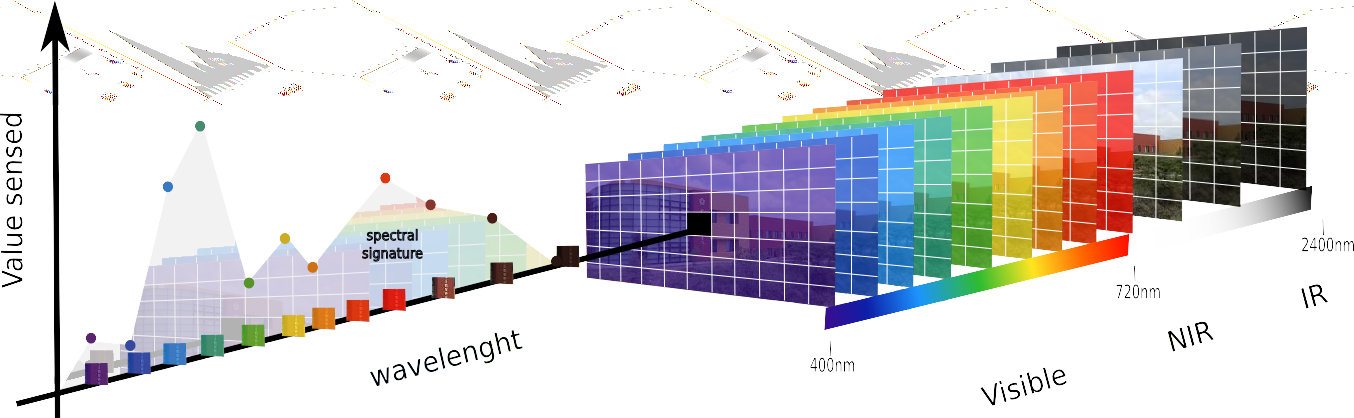
\includegraphics[width=.8\textwidth]{./images/jairo.png}}
  \centering
  \caption{Longitudes de onda \cite{FuzzyVD}.}
  \label{fJairo}
\end{figure}

\subsection{2.1.5 Imagen Hiperespectral}
El concepto de hiperespectral deriva de la toma de una gran cantidad de espectros de una superficie. Donde cada toma es tomada para formar un cubo de la imagen.(véase la Figura \ref{fWiki})

Tomando en cuenta la información recolectada a lo largo del espectro electromagnético se forma un cubo de datos con el que se puede trabajar ya según la aplicación que se le quiera dar. Usando los principios de \emph{Computed Tomography Image Spectrometes} (CTIS capítulo \ref{CTIS}), la forma en que se captura una imagen hiperespectral es obteniendo el contenido espectral de cada pixel en una imagen 2D superposicionada. Esta tecnología divide los datos de la imagen pixel por pixel en bandas estrechas de longitud de onda, dando como resultado un cubo 3D de datos como se muestra en la Figura \ref{fPaper1}.\\

\begin{figure}[h]
  \centering
  \framebox[9cm]{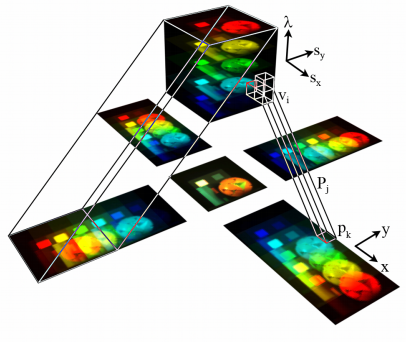
\includegraphics[width=.6\textwidth]{./images/paper1.png}}
  \centering
  \caption{Proyecciones paralelas de difracción \cite{PracCam}.}
  \label{fPaper1}
\end{figure}

\section{2.2 CTIS}
\label{CTIS}
Espectrómetro de imágenes por tomografía computarizada (en inglés \textit{Computed tomography imaging spectrometer} CTIS) es un método utilizado para la captura de las imágenes hiperespectrales sin necesidad de escaneo puesto que es obtenido en un snapshot que consiste en un único tiempo de integración gracias a un conjunto de detectores. 
Funciona como si se tratara de dos cámaras en sí, donde una toma la imagen base en un cuatro de visión y la segunda capta la energía a distintas longitudes de onda electromagnética reflectada en el marco tomado.
Dando como resultado una imagen de referencia(zero mode) y los espectros captados a diferentes longitudes de onda basadas en dicha imagen.

Da como resultado una imagen 2D que es una superposición de los espectros, siendo el cubo hiperespectral proyectado de forma paralela en distintos ángulos (vea la Figura \ref{fPaper1}). El cubo formado es compuesto por voxeles ($V_i$), que son una unidad cúbica componente de la imagen hiperespectral definidos por la resolución de la imagen superposicionada.   

La estructura del dispositivo CTIS son las presentadas en la Figura \ref{fCTIS}, donde la lente de imagen (imaging lens) refleja la imagen a través de la apertura ya sea una imagen o conjunto de imágenes (slit/square aperture). La luz divergente es hecha paralela al pasar por la lente de colimación (collimation lens), para después pasar por la rejilla de difracción (diffraction grating). La luz difractada y no difractada se vuelven a hacer imágenes mediante el lente de reimagen (re-imaging lens). Finalmente el resultante es captado por el sensor.

\begin{figure}[h]
  \centering
  \framebox[13cm]{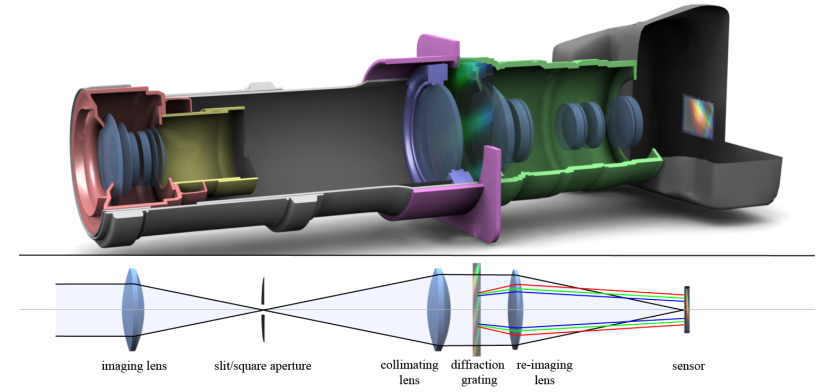
\includegraphics[width=.9\textwidth]{./images/CTIS.png}}
  \centering
  \caption{Estructura CTIS. \cite{PracCam}}
  \label{fCTIS}
\end{figure}

%Chapter 3 overview explain RGGB
\subsection{2.2.1 Calibración espacial}
%The spatial calibration localizes the positions of individual wavelenghts on the image grid (in slit mode), or determinesthe coefficients of the projection of the data cube.
%The calibration will allow a precise mapping from the projected image to wavelenghts in the spectrum.

La calibración espacial corrige distorsiones que tenga la imagen obtenida por el dispositivo CTIS. Lo que hace es buscar desalineamientos cuando pasa la luz entre la apertura (slit/square aperture) y la rejilla de difracción (diffraction grating).

\subsection{2.2.2 Calibración espectral}
%Calculates the spectral intensity response od the optical system and the sensor pixels. The pixels are arranged in a RGGB Bayer filter array, so each pixel responds more in the red, green or blue range of the spectrum. This means that similar to standard imaging, we need to apply demosaicing algorithms to recover the full spectra

El objetivo de la calibración espectral es ajustar la sensibilidad espectral de cada canal de color que se determinan identificando un espectro cuando es continuo y conocido con alta precisión.

\subsection{2.2.3 Medición de slit espectral e interpolación cromática}
Para la reconstrucción del verdadero espectro de la medición aplicando la calibración espectral {f(x,y)} debemos tomar en cuenta las diferentes sensibilidades de los diferentes canales de color en el filtro Bayer (Bayer filter \cite{Bayer}).
Cualquier canal puede ser utilizado para reconstruir un espectro considerando que se tiene una respuesta por cada canal de color.
Puesto que la respuesta espectral de cada canal cubre sólo parte del espectro visible y las posiciones de los píxeles de Bayer están entrelazadas, se combinan las mediciones de píxeles Bayer adyacentes con valores interpolados.
Para suprimir ruido los canales con peso (weight) $W_{r,g,b}(\lambda)$ donde $r,g,b$ corresponden a los colores rojo(red), verde(green) y azul(blue) basados en la amplitud de su respuesta espectral:
\begin{flalign}
  \label{FormulaMSS1}
  W_{r,g,b}(\lambda)=\frac{S_{r,g,b}(\lambda)}{\sum\limits_{c=r,g,b}S_{c}(\lambda)}.
\end{flalign}
después el espectro M($\lambda$) de una medida de respuesta $m_{r,g,b}(\lambda)$ es reconstruida con:
\begin{flalign}
  \label{FormulaMSS2}
  M(\lambda)=\sum\limits_{c=r,g,b}\frac{m_{c}(\lambda)}{S_{c}(\lambda)}w_{c}(\lambda)=\frac{\sum\limits_{c=r,g,b}m_{c}(\lambda)}{\sum\limits_{c=r,g,b}S_{c}(\lambda)}w_{c}(\lambda).
\end{flalign}
con valores interpolados donde fueron necesarios.


\subsection{2.2.4 Calibración hiperespectral}
La calibración hiperespectral consiste en usar la apertura cuadrada, puesto que tomando la apertura slit solo se podrá tener una imagen a una cierta longitud de onda. En cambio utilizando la apertura cuadrada se podrá tomar un conjunto de imágenes a lo largo del espectro electromagnético, logrando así el cubo de datos.
\subsubsection{2.2.4.1 Teoría de reconstrucción CTIS}
Para la reconstrucción se toma en cuenta una matriz $H$ generada por la proyección paralela (vea capítulo \ref{CTIS}) que trabaja con el vector $\vec{f}$ que contiene voxeles del cubo de datos como se mostró en la Figura \ref{fPaper1}. $H$ es una matriz $M x N$ donde $M$ es el número de píxeles en la imagen y $N$ el número de voxeles en el cubo de datos. Multiplicando la matriz por el vector $\vec{f}$ se obtiene un nuevo vector $\vec{g}$:
\begin{flalign}
  \label{FormulaCH1}
  \vec{g}=H\vec{f}.
\end{flalign}
Cada columna contiene cinco entradas en la en las posiciones difractadas en el centro (zero mode). Como resultante de lo mencionado la matriz $H$ es muy grande por lo que se invierte la ecuación \ref{FormulaCH1}. Con la matriz $H$ se genera una primera suposición a través de $\vec{\hat{f}}0=H^T\vec g$ y se realiza la etapa iterativa de maximización de expectativas:
\begin{flalign}
  \label{FormulaCH2}
  \hat{f}_{n}^{k+1}=\frac
            {
              \hat{f}_{n}^{k}
            }
            {
              \sum\limits_{m=1}^{M}H_{mn}
            }
            \sum\limits_{m=1}^{M}
              H_{nm}^{T}
            \frac
            {
              g_{m}
            }
            {
              (H\hat{f}^{k})_{m}
            }.
\end{flalign}

\subsubsection{2.2.4.2 Calibración espacial hiperespectral}
Para calibrar la imagen hiperespectral se deberán tener identificadas las proyecciones correspondientes a cada espectro en las cinco entradas. Con base en la Figura \ref{fPaper1} se identificada la correspondencia de las proyecciones con base en las coordenadas $(x,y)$ de la imagen plana. 
Si se deja a $P_{j}$ como proyecciones del cubo de datos $P_{j}(s_{x},s_{y},\lambda) = (x,y)$ construido por los voxeles $v_{i}=(s_{x_{i}},s_{y_{i}},\lambda_{i})$ que da cinco píxeles $p_k=(x_k,y_k)$ con índices $k \in 1...M$. Entonces $H$ puede ser construido mediante las cinco entradas $p_{k_1},...,p_{k_5}$ en la i-ésima columna de $H$ a uno.

Para que esto suceda se necesita determinar la posición de las cinco proyecciones para identificar alguna inclinación que tenga la imagen y poderlo revertir. Se toma una captura siendo $P_{0}$ el modo zero y $P_{1..4}(s_x,s_y,\lambda) = (x,y)$ (vea Figura \ref{fPaper1}), se alinean las $P_{1..4}$ en forma de cruz tomando como referencia central a $P_{0}$ mediante una interpolación lineal. 

\subsubsection{2.2.4.3 Medición de imágenes hiperespectrales}
Al tener una imagen hiperespectral CTIS se necesita hacer una medición de las señales a distintas longitudes de onda para de esta forma identificar las caractarísticas superposicionadas de las diversas longitudes de ondas del espectro electromagnético.

Teniendo la matriz $H$ definida se puede proseguir para la solución de una imagen CTIS. Considerando que la utilizando la ecuación \ref{FormulaCH2} da una gran cantidad de ceros se tienen datos y procedimientos innecesarios. Para solucionar esto se propone separar por canal el arreglo de imagen Bayer tratando a los dos canales de verde (green G) del arreglo Bayer RGGB. Se realiza lo mismo con la matriz H para extraer H matrices para cada uno de los cuatro canales (RGGB) solo para las longitudes de onda donde la correspondencia no sea cero.

\subsubsection{2.2.4.4 Interpolación cromática espacial y reconstrucción}
\label{Reconstruction}
La interpolación cromática (demosaicing) es el proceso que se realiza a un conjunto de muestras cromáticas tomadas de un sensor de imagen para producir una imagen a color.
Una vez realizada la interpolación cromática se podrá hacer la reconstrucción en la imagen CTIS.
Para realizar la reconstrucción se realiza una interpolación cromática, similar a la interpolación cromática con imágenes RGB. 
Posterior a ello se hace una interpolación bilineal para obtener los píxeles Bayer. 
Una interpolación cromática espectral es diferente a las convencionales, por su información en superposición contenida.
Con el cubo de datos interpolados cromáticamente se recuperan los píxeles espectrales utilizando la ecuación \ref{FormulaMSS1}. 
Mediante la configuración slit se recolectan los valores por espectro, provocando de esta forma una integral para calcular la información en 
$S_{r,g,b}^l(\lambda_i)$
en resoluciones bajas:
\begin{flalign}
  \label{FormulaSDR}
  S_{r,g,b}^l(\lambda_i)=\int _{\lambda_i-\frac{r}{2}}^{\lambda_i+\frac{r}{2}}S_{r,g,b}(\lambda)d\lambda.
\end{flalign}


\section{2.3 Mosaico de Bayer\cite{Bayer}}
El mosaico de Bayer es la interpolación en la imagen de dos muestras verdes, una roja y otra azul. Se tomó en cuenta el patrón Bayer RGGB dejando en porcentaje 50\% de filtros verdes, un 25\% de rojos y un 25\% de azules en la imagen. La razón por la que se utilizan más muestras verdes es porque el ojo humano es más sensible a ese color.

Siendo el verde que aparece en todas las filas, los colores azul y rojo aparecen por fila uno y después el otro, denominando la fila roja cuando tiene rojo y verde, y fila azul cuando tiene azul y verde. Los verdes pueden aparecen en la posición par o la impar, alterado por el color de fila que se encuentre.
La fila con rojo tendría el patrón rojo, verde,rojo,verde,..., y el la fila con azul el patrón verde, azul, verde, azul,...

El patrón esta desplegado en la Figura \ref{fBayer}.

\begin{figure}[h]
  \centering
  \framebox[9cm]{\includegraphics[width=.6\textwidth]{./images/bayer.png}}
  \centering
  \caption{Patrón de Bayer.}
  \label{fBayer}
\end{figure}
%\subsection{Pseudocódigo}

%aplicado a imágenes wavelets0.
\section{2.4 Método de Malvar, He y Cutler}\label{capMalvar}
El método propuesto por Malvar, He y Culter deriva de una modificación de la interpolación bilineal e intenta atacar los problemas de la interpolación cromática. El algoritmo propuesto consta de un simple método lineal usando filtros 5x5. Para la interpolación cromática se utilizará la imagen pasada por una matriz de filtros de color (en inglés \textit{Color Filter Array} CFA) Bayer pattern\cite{Bayer}.

En localización del azul o rojo pixel, la interpolación bilineal del componente verde es el promedio de sus cuatro vecinos axiales,
\begin{flalign}
  \label{Malvar1}
  \hat{G}^{bl}(i,j)=
  \frac{1}{4}(
  G(i-1,j)+
  G(i+1,j)+
  G(i,j-1)+
  G(i,j+1)
  ).
\end{flalign}
La interpolación bilineal de los componentes azul y rojo son similares, la diferencia es que toman a sus cuatro vecinos diagonales.

La localización del componente verde en el pixel rojo está estimado como
\begin{flalign}
  \label{Malvar2}
  \hat{G}(i,j)=\hat{G}^{bl}(i,j)+\alpha \Delta _R(i,j),
\end{flalign}
donde $\Delta _R$ es el Laplaciano discreto de cinco puntos del canal rojo,
\begin{flalign}
  \label{Malvar3}
  \Delta _R(i,j):=R(i,j)-\frac{1}{4}(R(i-2,j)+R(i+2,j)+R(i,j-2)+R(i,j+2)).
\end{flalign}
Para estimar el componente rojo en la lo localización del pixel verde,
\begin{flalign}
  \label{Malvar4}
  \hat{R}(i,j)=\hat{R}^{bl}(i,j)+\beta \Delta _G(i,j),
\end{flalign}
donde $\Delta _G$ es el Laplaciano discreto de nueve puntos del canal verde.
Para estimar un componente rojo en una localización de un pixel azul,
\begin{flalign}
  \label{Malvar5}
  \hat{R}(i,j)=\hat{R}^{bl}(i,j)+\gamma \Delta _B(i,j),
\end{flalign}
donde $\Delta _B$ es el discreto Laplaciano de cinco puntos del canal azul.

Los parámetros de $\alpha$, $\beta$ y $\gamma$ controlan el peso de los términos de conección Laplacianos, 
\begin{flalign}
  \label{Malvar6}
  \alpha =\frac{1}{2},\text{  }\beta =\frac{5}{8},\text{  }\gamma \frac{3}{4}.
\end{flalign}


\section{2.5 Gaussian blur\cite{Blur}}\label{CapBlur}
El desenfoque Gaussiano (Gaussian blur) es un método que utiliza algorítmos matemáticos. Se basa en la función Gaussiana,
\begin{flalign}
  \label{Gauss1}
  f(x)=ae-\frac{{(x-b)}^2}{2c^{2}}
\end{flalign}
que aplicado a las imágenes mezcla poco los colores de los vecinos de los píxeles entre sí. Lo cual ocasiona que se pierdan detalles y se vea incluso borroso. 
Para la aplicación de esta función en las imágenes utilizadas en el proyecto se utilizó matlab.

\section{2.6 Sharpender\cite{Sharp}}\label{capSharpender}
La nitidez(sharpender) es el proceso inverso a desenfoque, puesto que intenta dar forma a bordes y a detalles de la imagen.
Pretende dar más calidad en la imagen resaltando pequeños contrastes en los píxeles con respecto a sus vecinos.
Para la aplicación de esta función en las imágenes utilizadas en el proyecto se utilizó matlab.
\section{2.7 GPA}
El algorítmo Análisis General Anterior(en inglés \textit{General Analysis Prior} GAP) para la reducción de ruido impulsivo para imágenes hiperespectrales esta basado en la minimización de la variación total.
\subsection{2.7.1 Transformada de Fourier}
Las transformadas de Fourier han jugado un papel importante al referirse a algoritmos de reconstrucción y filtrado de imágenes. A continuación se dará un repaso a las series de Fourier que después serán referenciadas en uno de los algoritmos de filtrado de imágenes utilizado en el presente proyecto.
\subsubsection{2.7.1.1 Series de Fourier \cite{FourierBook}}
Una función periódica $g(x)$ con un periodo $T$ tal que
\begin{flalign}
	\label{Fourier1}
	g(x)=g(x+T), -\infty  < x < \infty 
\end{flalign}
podrá ser representada como una serie de Fourier:
\begin{flalign}
	\label{Fourier2}
	g(x)=\sum \limits_{n=-\infty}^{\infty}G_{n}e^{\frac{i2\pi nx}{T}}.
\end{flalign}
La función $g(x)$ deberá ser integrable en un periodo y ser continua. La función $g(x)$ deberá tener extremos en un periodo.
El coeficiente $G_{n}$ puede ser determinado por la siguiente relación ortogonal:
\begin{flalign}
	\label{Fourier3}
	\int_{-\frac{T}{2}}^
	{\frac{T}{2}}
	dx\text{ }
	e^{\frac{i2\pi (m-n)x)}{T}}
	=
	\left [ 
	\frac
	{e^{\frac{i2\pi (m-n)x)}{T}}}
	{\frac{i2\pi (m-n))}{T}}
	\right ]_
	{-\frac{T}{2}}^
	{\frac{T}{2}}=
	T \frac{\sin \pi (m-n))}{\pi (m-n))}=
	T\delta _{m,n}
\end{flalign}
Los coeficientes $G_n$ pueden ser obtenidos como:
\begin{flalign}
	\label{Fourier4}
	G_n=\frac{1}{T}\int _{-\frac{T}{2}}^{\frac{T}{2}}dx\text{ }g(x)e^{\frac{-i2\pi nx}{T}}.
\end{flalign}
Si g(x) tiene una discontinuidad en $x=x_0$, la expanción de la serie converge a:
\begin{flalign}
	\label{Fourier5}
	g(x_0)=\frac{g(x_{0-})+g(x_{0+})}{2}.
\end{flalign}
Todos los términos impares son utilizados, por lo que la expansión de la serie de Fourier queda así:
\begin{flalign}
	\label{Fourier6}
	g(x)=\frac{1}{2}+\frac{2}{\pi}sin(\frac{2\pi x}{T})+\frac{2}{3\pi}sin(\frac{6\pi x}{T})+...
\end{flalign}
Las tramas producidas por la serie converge a una onda cuadrada. En la Figura \ref{fFourier} se puede ver como al agregar más términos de la serie se produce la convergencia. 

\begin{figure}[h]
  \centering
  \framebox[9cm]{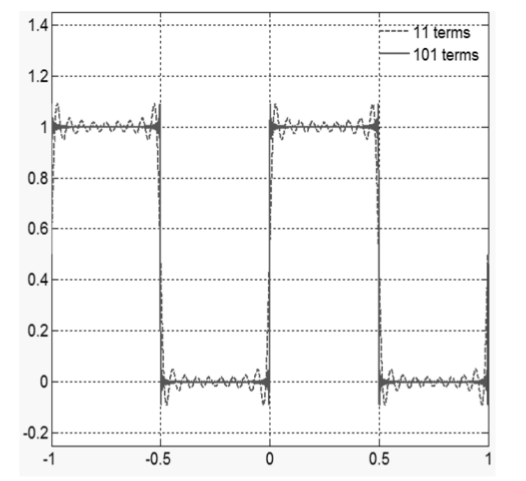
\includegraphics[width=.6\textwidth]{./images/fourier.png}}
  \centering
  \caption{Onda cuadrada representación de serie de Fourier con 11 y 101 terminos como en la ecuación \ref{Fourier6} \cite{FourierBook}.}
  \label{fFourier}
\end{figure}

%\subsubsection{Fenómeno de Gibbs}

\subsection{2.7.2 Transformadas de Wavalet}
Las wavelets son prácticamente mini ondas a diferencia de las infinitas como seno y coseno. La finalidad de que sean cortas es que puedan desvanecer rápidamente, limitadas en tiempo y frecuencia. A diferencia de la transformada de Fourier siendo infinita, la transformada de Wavalet es desarmada usando el mismo wavalet a diferentes escalas en vez de usar la misma frecuencia de seno vea Figura \ref{fWvsF}.

\begin{figure}[h]
  \centering
  \framebox[9cm]{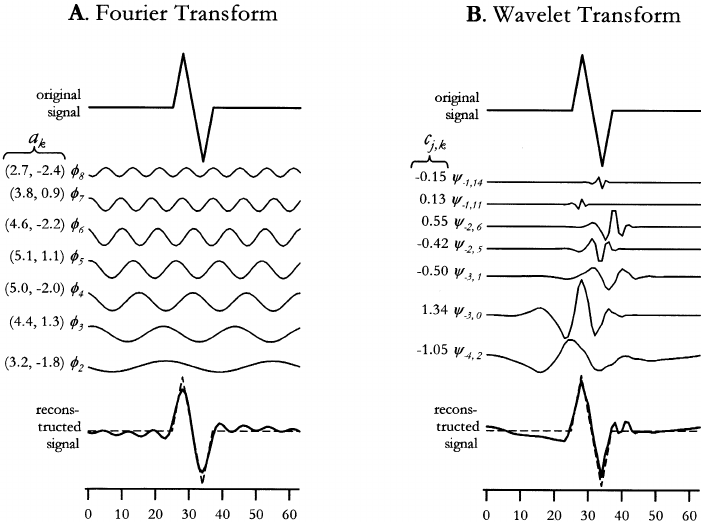
\includegraphics[width=.6\textwidth]{./images/waveletvsfft.png}}
  \centering
  \caption{Comparación entre transformada de Fourier y Wavelet \cite{WaveVsFourier}.}
  \label{fWvsF}
\end{figure}

Llamese $\varphi$ una base ortogonal del subespacio por escalación y transición se presenta la ecuación 

\begin{flalign}
	\label{Dau1}
	\varphi _{i,j}(t)=\frac{1}{\sqrt{2}}\sum_{k\in \mathbf{Z}}h_k\varphi_{j+1,k}(t),
\end{flalign}

 siendo las funciones wavelets $\psi_{i,k}(t)$,  donde

 \begin{flalign}
	\label{Dau2}
	\psi_{i,k}(t)=\frac{1}{\sqrt{2}}\sum_{k\in \mathbf{Z}}g_k \varphi_{i+1,k}(t).
\end{flalign}

Se puede definir una transformada Wavelet como $f(t)$, donde

 \begin{flalign}
	\label{Dau3}
	f(t)=\sum_{j=0}^{J-1}\sum_{k=0}^{2^j-1}\omega _{j,k}\psi_{J,k}(t)+\sum_{k=0}^{L-1}s_{J,k}\varphi_{J,k}(t).
\end{flalign}

\subsubsection{2.7.2.1 Daubechies}\label{rDau}%http://wwwmayr.in.tum.de/konferenzen/Jass05/courses/2/Yakovlev/Yakovlev_paper.pdf
Para obtener las transformadas Daubechies es necesario aplicar condiciones de momentos nulos(zero moments) a la función Wavelet que se le llamará función padre. Para hacer esto se deberán tener presentes las siguientes condiciones:

\begin{flalign}
  \label{Dau3}
  \left\{\begin{matrix}
  h_0+h_1+h_2+h_3=\sqrt{2}
  \\ h_1+2h_2+3h_3=0
  \\ h_0^2+h_1^2+h_2^2+h_3^2=1
  \\ h_0h_2+h_1h_3=0
\end{matrix}\right.
\end{flalign}
donde las soluciones serían:
\begin{flalign}
	\label{Dau3}
	h_0=\frac {1+\sqrt{3}}{4\sqrt{2}},\text{  }
	h_1=\frac{3+\sqrt{3}}{4\sqrt{2}},\text{  }
	h_2=\frac{3-\sqrt{3}}{4\sqrt{2}},\text{  }
	h_3=\frac{1-\sqrt{3}}{4\sqrt{2}}.
\end{flalign}

En la Figura \ref{fDau} se puede observar un ejemplo de wavelength aplicando las condiciones de momentos nulos en contraste con una función general wavelet.

\begin{figure}[h]
  \centering
  \framebox[9cm]{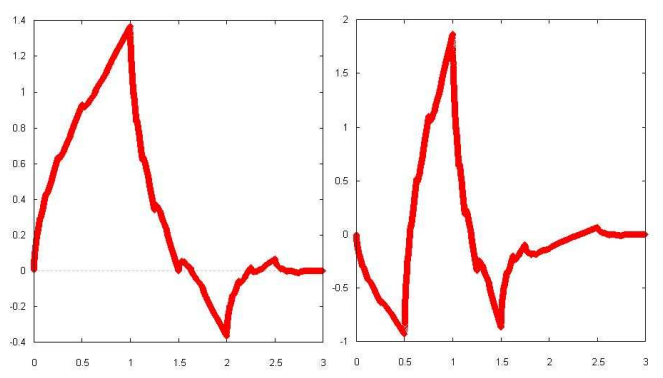
\includegraphics[width=.6\textwidth]{./images/dau.png}}
  \centering
  \caption{Daubachies y función wavelet \cite{Yakovlev}.}
  \label{fDau}
\end{figure}
%http://wwwmayr.in.tum.de/konferenzen/Jass05/courses/2/Yakovlev/Yakovlev_paper.pdf

